\documentclass[11pt,letterpaper]{article}

\usepackage[letterpaper,margin=0.8in,nohead]{geometry}

\usepackage[colorlinks]{hyperref}
\usepackage{url}
\usepackage{breakurl}

\hypersetup{
	colorlinks,
	linkcolor={red},
	citecolor={red},
	urlcolor={blue}
}

\usepackage{verbatim}
\usepackage{fancyvrb} 
\usepackage{scrextend}
\usepackage{enumitem}
\usepackage{url}
\usepackage{tabularx}

\usepackage{caption}
\usepackage{graphicx}
\usepackage{subcaption}

\usepackage{changepage}   % for the adjustwidth environment

\newenvironment{answer}{\em \color{blue} \begin{adjustwidth}{1cm}{1cm}}{\end{adjustwidth}}

% math
\usepackage{amsthm,amsmath}
\usepackage{amsfonts}

\newcommand{\mc}[1]{\mathcal{#1}}	% Mechanisms / Algorithms
\newcommand{\rv}[1]{\mathbf{#1}}    % Random variable

\newcommand{\pr}[1]{\mathrm{Pr}\{#1\}} % Probability

\newtheorem{corollary}{\bf Corollary}%[theorem]
\newtheorem{lemma}{\bf Lemma}%[theorem]
\newtheorem{definition}{\bf Definition}%[section]

\newtheorem{observation}{\bf Observation}%[theorem]

% load cleveref last!
\usepackage[capitalise]{cleveref}


\begin{document}
	
	\title{EN4720: Security in Cyber-Physical Systems \\ Exercise --- Authentication}
	
	%% This is an individual assignment!!
	%% TODO: put your name and index number here here!
	\author{ \textcolor{blue}{Name: Thalagala B. P.} \\ \textcolor{blue}{Index No: 180631J}}
	
	\maketitle
	
	\begin{center}
		\color{red}\bf This is an individual exercise! \\ Due Date: 19 May 2023 by 11.59 PM
	\end{center}
	
	\begin{center}
		\small Content adopted from the Udacity Security Engineer Nano-Degree and ECU CSI 1101.    
	\end{center}
	
	\vspace{1in}
	
	This exercise has to be carried out using a Linux-based PC/virtual machine. Read all the instructions and questions before attempting the exercise. Add answers under each question in the Questions section and submit the resulting PDF. All files used in this exercise can be found in {\it ex3-resources} folder.
	
	\subsection*{Instructions}
	
	\begin{enumerate}
		\item Explore and understand how Unix systems store and manage passwords.
		
		\item Download the shadow.hex file from the ``files'' folder. This file has been encrypted using RC4 encryption. 40 bits hexadecimal key: \textcolor{magenta}{5D 49 34 71 64}. Decrypt the file using any available decryption tool (e.g., cryptool).
		
		\item Download the ``500\_passwords.txt'' file from the “files” folder. Run ``hashcat'' password cracking utility to crack the passwords in the decrypted shadow file with the help of the dictionary ``500\_passwords.txt''. Please note that, to crack the passwords in the decrypted shadow file using hashcat, you need to take encrypted password fields of each user into a different file. You may rename that file as ``encrypted\_passwords.txt''.
		
		\item Download the ``myhashes.txt'', ``mydictionary.txt'', ``myruleset.txt''  files from the “files” folder. Note that, myhashes.txt containes MD5 hashes. Run a rule-based attack using “hashcat” password cracking utility to crack the passwords in the myhashes.txt file with the help of the dictionary “mydictionary.txt” and the ruleset myruleset.txt.
		
		\item Answer the questions given below.
		
	\end{enumerate}
	
	\newpage
	\subsection*{Questions}
	
	\begin{enumerate}
		
		\item What is the difference between \textcolor{magenta}{/etc/passwd} and \textcolor{magenta}{/etc/shadow} files? Complete Table~\ref{tab:difference-passwd-shadow}.
		
		\begin{answer}
			\textcolor{magenta}{/etc/passwd} file stores the account details of the users on a given host machine. The content of the file is word-readable and everyone has the read permission for that file. 
			
			\begin{verbatim}
			(user@host)-[/etc]
			$ ls -lh | grep passwd
			-rw-r--r--  1 root root   2.0K Apr  2 14:44 passwd
			-rw-r--r--  1 root root   2.0K Apr  2 14:38 passwd-
			\end{verbatim}
		
			\textcolor{magenta}{/etc/shadow} file stores the details about the passwords of users and encrypted passwords. The shadow file can only be read by the root account.
			
			\begin{verbatim}
			(user@host)-[/etc]
			$ ls -lh | grep shadow
			-rw-r-----  1 root shadow  770 Apr  2 14:44 gshadow
			-rw-r-----  1 root shadow  761 Apr  2 14:44 gshadow-
			-rw-r-----  1 root shadow  968 Apr  2 14:44 shadow
			-rw-r-----  1 root shadow  949 Apr  2 14:38 shadow-
			\end{verbatim}
			
			\begin{table}[h!]
				\caption{Difference between /etc/passwd amd etc/shadow files} \label{tab:difference-passwd-shadow}
				\begin{tabularx}{\columnwidth}{|p{4cm}|X|X|}
					\hline
					\textbf{Attribute} & \textbf{/etc/passwd} & \textbf{etc/shadow} \\
					\hline
					Number of fields & 7 & 9\\\hline
					
					\hline
					Accessible users & Anyone can read& Only {\tt root} user and members of {\tt shadow} group can read \\\hline
				\end{tabularx}
			\end{table}
			
		\end{answer}
		
		
		
		\item You will find seven fields in the /etc/passwd file as indicated in Figure~\ref{fig:etc-passwd-format}. Explain the purpose of each field.
		
		\begin{figure}[h]
			\centering
			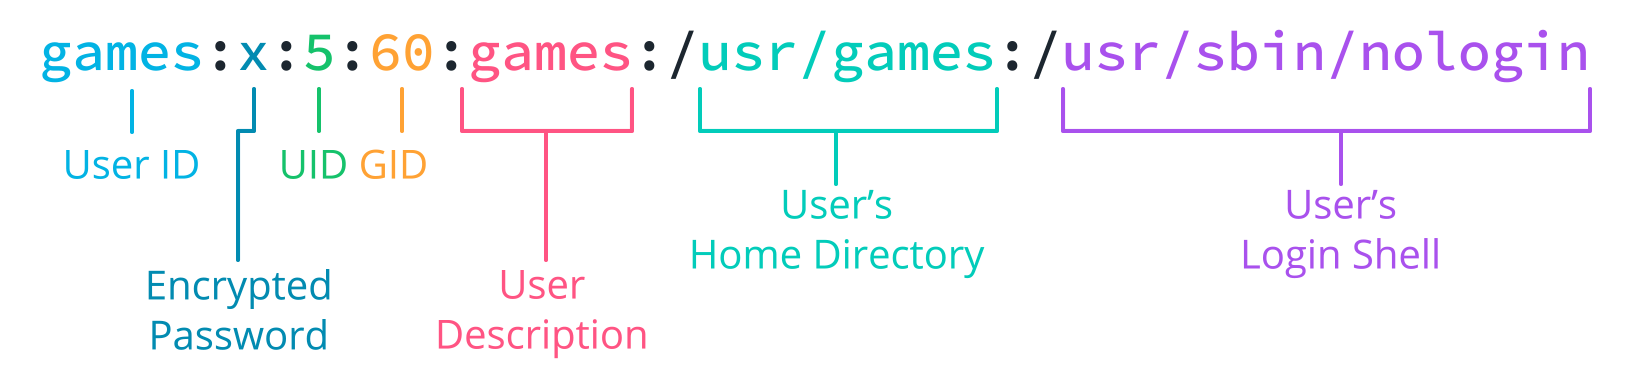
\includegraphics[width=0.65\columnwidth]{images/ex3-etc-passwd-format.png}
			\caption{Example storage format of /etc/passwd file} \label{fig:etc-passwd-format}
		\end{figure}
		
		\begin{answer}
			\begin{enumerate}
				\item \textbf{games}: name of the user for whom this entry corresponds to.
				\item \textbf{x} : indicates that a password exists for the user. However, the password is stored in the \textcolor{magenta}{/etc/shadow} file. If instead of x it shows a ! symbol, this indicates that a password does not exist.
				\item \textbf{5} : User ID of this user. User IDs for created users begin from 1000 and run up to 59999
				\item \textbf{60}: Group ID of the group this user belongs to.
				\item \textbf{games}: indicates multiple comma separated fields of information inclusive of full name and telephone numbers. Here, no telephone numbers have been provided.
				\item \textbf{/usr/games} : location of home directory assigned to this user.
				\item \textbf{/usr/sbin/nologin} : default shell assigned to this user.
			\end{enumerate}
			
			
			
		\end{answer}
		Note: Information adopted from,  \\\url{https://www.maketecheasier.com/how-linux-stores-manages-user-passwords/}
		
		
		
		\item Dump the content of your /etc/shadow file to the terminal using \textcolor{magenta}{sudo cat /etc/shadow} and add a screenshot.
		
		\begin{answer}
			%% TODO: Add answer here
			Your answer here
		\end{answer}
		
		\item Identify the different fields present in one line in the shadow file and explain the purpose of each field. Clearly mark the fields and provide the explanation.
		
		\begin{answer}
			%% TODO: Add answer here
			Your answer here
		\end{answer}
		
		\item Complete Step \#2 mentioned under \textbf{Instructions}. Add a screenshot of the decrypted shadow.hex file content. What is the type of hash in the decrypted shadow file?
		
		\begin{answer}
			%% TODO: Add answer here
			Your answer here
		\end{answer}
		
		\item Complete Step \#3 mentioned under \textbf{Instructions}. Add a screenshot of a part of the ``500\_passwords.txt'' file content using vi/vim/nano.
		
		\begin{answer}
			%% TODO: Add answer here
			Your answer here
		\end{answer}
		
		\item What is the command you used to crack the passwords in the shadow file? Briefly explain each field in the command.
		
		\begin{answer}
			%% TODO: Add answer here
			Your answer here
		\end{answer}
		
		\item Add a screenshot of all the cracked passwords.
		
		\begin{answer}
			%% TODO: Add answer here
			Your answer here
		\end{answer}
		
		\item Provide recommendations to enhance the strength of the passwords.
		
		\begin{answer}
			%% TODO: Add answer here
			Your answer here
		\end{answer}
		
		\item Briefly explain about ``Rule-based Attack'' and how it uses time and memory for the hash cracking process using a diagram.
		
		\begin{answer}
			%% TODO: Add answer here
			Your answer here
		\end{answer}
		
		\item Complete Step \#4 mentioned under \textbf{Instructions}. Add a screenshot of the mydictionary.txt and myruleset.txt file contents. Define each rule in myrulset.txt using standard rules in the rule-based attack.
		
		\begin{answer}
			%% TODO: Add answer here
			Your answer here
		\end{answer}
		
		\item Add a screenshot of all the cracked passwords. Run a dictionary attack without myruleset.txt (using only the dictionary) and compare the two cracked files.
		
		\begin{answer}
			%% TODO: Add answer here
			Your answer here
		\end{answer}
		
	\end{enumerate}
	
\end{document}